\chapter{Theoretical background}



\section{Planetary orbits and approximations analysis}
In order to calculate the interplanetary trajectory between two planets, several approximations can be used. The simplest approximation, which can be called \textit{aprox. 0} accepts the following hypothesis: 
\begin{itemize}
\item Circular and coplanar orbits
\item No analysis about the exit of the planet of start is done.
\item No analysis about entering the planet of arrival is done. 
\end{itemize} 
\textit{Aprox. 0} is very basic and can be easily improved adding some parameters.\\
Another approximation widely used is \textbf{Patched Conic Approximation (PCA)}. This method improves significantly the results obtained with \textit{aprox. 0} and represents a good starting point for a more precise numerical analysis of the mission. For this reason, in this project the PCA method will be used. 
\subsection{Patched Conic Approximation (PCA)}
The Patched Conic Approximation (PCA) consist on the evaluation of an interplanetary trajectory dividing it into three stages. Considering the Earth as the planet of start, this stages are: 
\begin{itemize}
\item Geocentric phase: Hyperbolic exit of the Earth. This phase takes place while the probe is going through the influence sphere of the Earth. 
\item Heliocentric phase: Trajectory with the Sun as main influencer.
\item Planet-centred phase: Hyperbolic arrival to the planet of destination. Similarly to the geocentric phase, this phase starts when the probe enters the sphere of influence of the planet. 
\end{itemize}
The influence spheres mentioned are the space close to the planets where it can be considered that the influence of the Sun is negligible in comparison with that of the planet in question. The Laplace criteria will be considered to calculate this sphere. In Table \ref{RIplanets} the radius of the sphere of influence of the solar system's planets are shown. 
\begin{table}[H]
\centering
\begin{tabular}{|lccc|}
\hline
Planet  & $R_I\times 10^6 $km & $R_I\times 10^{-3} $ UA & $R_I$ Radius of the planet \\ \hline
Mercury & 0.111                       & 0.740                        & 45                     \\
Venus   & 0.616                       & 4.11                         & 100                    \\
Earth   & 0.924                       & 6.16                         & 145                    \\
Mars    & 0.577                       & 3.85                         & 170                    \\
Jupiter & 48.157                      & 321.0                        & 677                    \\
Saturn  & 54.796                      & 365.3                        & 901                    \\
Uranus  & 91.954                      & 346.4                        & 2025                   \\
Neptune & 80.196                      & 534.6                        & 3866                   \\ \hline
\end{tabular}
\caption{Radius of influence of the planets}
\label{RIplanets}
\end{table}
In order to set out the problem and begin with the resolution of it using the PCA method, the times and positions of the planets at the beginning and end of the trajectory are needed and some hypothesis are taken under consideration. The hypothesis are: 
\begin{itemize}
\item The spheres of influences of the planets are not considered during the heliocentric phase. This hypothesis is admissible because the radius of the sphere are very small in comparison with the distance between planets.
\item The spheres of influence are considered infinite from the point of view of the planet. This is assumed due to the fact that the radius of influence of the planets are much larger than the radious of the planet itself, as can be seen in Tabl \ref{RIplanets}.
\item The duration of the trajectory can be taken as the duration of the heliocentric phase. 
\end{itemize}
 With this data the trajectory can be found through the orbital elements of the trajectories and the thrust required. 

\subsubsection{1st. Geocentric stage }
This first stage of the trajectory of the probe aims to escape the gravitational field exerted by the departure planet. To achieve this, it is necessary to follow a hyperbolic trajectory that guarantees to pass through the planet sphere of influence with a relative velocity $V_\infty$ (also known as hyperbolic excess velocity).

Therefore, in this section necessary equations to characterize this hyperbole will be reviewed. Figure~\ref{fig:HyperParam} shows the aforementioned situation. From the figure, it can be inferred that the hyperbola is defined by:
\begin{itemize}
	\item \textit{C}: Center of the hyperbola.
	\item $beta$: Angle of the hyperbola.
	\item \textit{b}: Exit parameter.
\end{itemize} 

\begin{figure}[H]
	\centering
	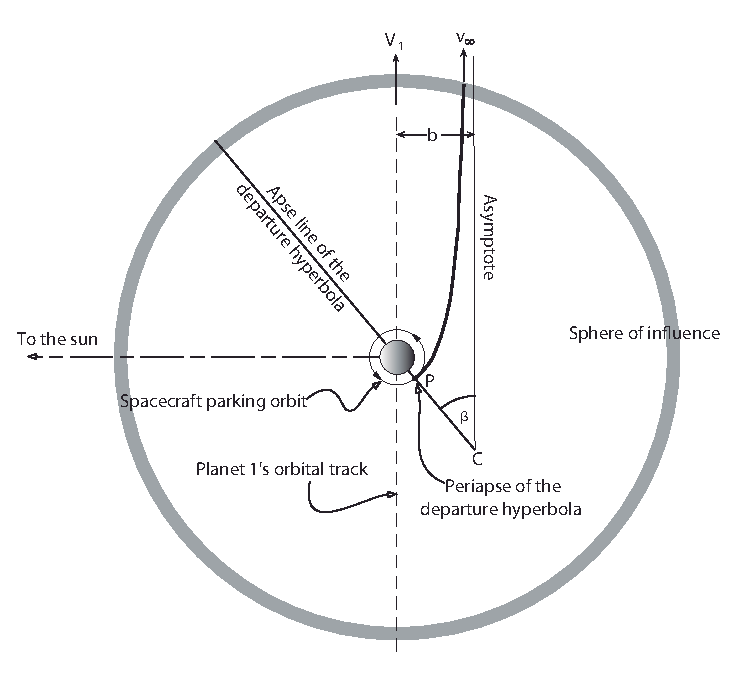
\includegraphics[width=0.5\textwidth]{././images/1stStage1} 
	\caption{Hyperbola Parameters. Extracted from~\cite{llibreVictor}.}
	\label{fig:HyperParam}
\end{figure}

The hyperbola can also be defined by the semi-major axis (\textit{a}) and the eccentricity (\textit{e}). In addition, the $\Delta V$ necessary to inject the probe into the hyperbolic orbit from the parking orbit must be specified.

To obtain these parameters, only the heliocentric departure speed ($v_1$), the velocity of the departure planet ($v_p$) and the parking orbit (in particular, the periapse radius and the speed of the orbit) are needed.


\paragraph{Definition of hyperbola:}
The first step is to obtain the semi-major axis of the hyperbola. This is obtained from the hyperbolic excess velocity as:
\begin{equation}
	a = \frac{\mu}{V_\infty^2}
\end{equation}

where $\mu$ is the standard gravitational parameter ($\mu=GM$) for the sun and the excess velocity is computed as the difference between the probe velocity and the departure planet speed. The eccentricity of hyperbola is defined by:
\begin{equation}
	e=1+(\frac{V_\infty}{V_0})^2
\end{equation}
where $V_0$ refers to the speed of the parking orbit. If this orbit is assumed to be circular with $r_0$ as the periapse, the probe velocity through the parking orbit is given by:
\begin{equation}
	V_0=\sqrt{\mu_0/r_0}
\end{equation}

being $\mu_0$ the standard gravitational parameter of the departure planet. Once the eccentricity is computed, the beta angle is easily obtained as:
\begin{equation}
	\cos \beta = \frac{1}{e}
\end{equation}

Finally, the exit parameter is computed by means of:
\begin{equation}
	b=a\sqrt{e^2-1}
\end{equation}

Obtaining the center of the hyperbola is a little bit more cumbersome. Given the three velocities ($V_\infty$, $v_p$ and $v_1$), the two frames of the figure~\ref{fig:frames} can be defined. One has the Y-axis in the direction of the planet velocity and the other has the vernal point over the X-axis. Then, the angle between the planet velocity and this X-axis is defined as $\lambda_v=90+\lambda_x$. Determining this $\lambda_x$ at the injection time $t_1$ 
allows us to obtain the right ascension ($\alpha$) and the declination ($\delta$) of the $v_1$ velocity by means of a change of frame:
\begin{equation}
	\left[\vec{V_\infty}\right]_\mathcal{Q}=\mathcal{R}_1(-\varepsilon)\mathcal{R}_3(-\lambda_x)	\left[\vec{V_\infty}\right]_\mathcal{K}
\end{equation}
Thus,
\begin{equation}
	\sin \delta =\left[V_z\right]_\mathcal{Q}; \qquad \tan \alpha=\left[\frac{V_y}{V_x}\right]_\mathcal{Q}
\end{equation}
Finally, the center of the hyperbola has the following coordinates ($\alpha+12^h$, $\delta$).
\begin{figure}[H]
	\centering
	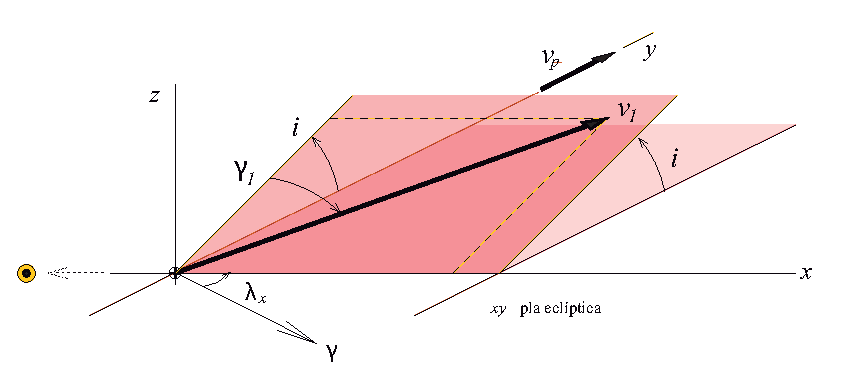
\includegraphics[width=0.5\textwidth]{././images/1stStage2} 
	\caption{Velocities frames of reference. Extracted from~\cite{PCA}}
	\label{fig:frames}
\end{figure}
\paragraph{Delta-v determination}
The necessary delta-v to put the probe onto the hyperbolic departure trajectory is given by:
\begin{equation}
	\Delta V=v_p-V_0=\sqrt{V_\infty+2V_0}-V_0
\end{equation}
The only requirement of the plane of the departure hyperbola is that it must contain the planet center of mass as well as the hyperbolic excess velocity. Therefore, the delta-v has to be applied once the probe flies over C, at a distance of $r_0*\sin \beta$. The circle of all the possible perigees is the injection points circle.
\begin{figure}[H]
	\centering
	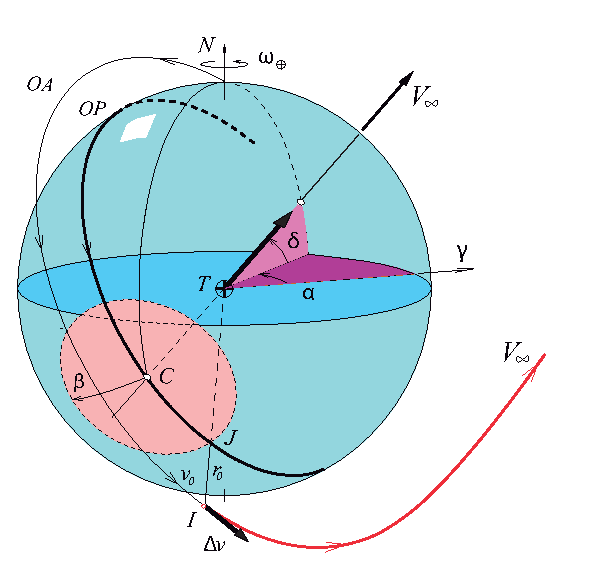
\includegraphics[width=0.5\textwidth]{././images/1stStage3} 
	\caption{Injection points circle. Extracted from~\cite{PCA}}
\end{figure}



\subsubsection{2nd. Heliocentric stage }
In this section the equations and assumptions done in order to obtain the orbital elements of the trajectory will be explained. The objective of the calculations done regarding this stage is to find:
\begin{itemize}
\item $\Omega$ : Right ascension of the ascending node.
\item \textit{e}: Eccentricity.
\item \textit{i}: Inclination to the ecliptic plane.
\item \textit{a}: Semimajor axis.
\item $\omega$ : Argument of the perihelion. 
\end{itemize} 
As said previously, the times of departure and arrival are provided, together with the position of the planets. The steps to be followed to achieve the aim of this section are now explained.
\paragraph{Longitude, latitude and distance}
The position vector is defined as: 
\begin{equation}
\overrightarrow{r}=\left( x_k, y_k, z_k \right)
\end{equation}
Where: 
\begin{equation}
x_k = r cos\beta cos\lambda
\end{equation}
\begin{equation}
y_k=r cos\beta sin\lambda
\end{equation}
\begin{equation}
z_k=r sin\beta
\end{equation}
Then longitude, latitude and distance are computed with: 
\begin{equation}
r=|\overrightarrow{r}|
\end{equation}
\begin{equation}
\beta = \arcsin\left(\frac{z_k}{r}\right)
\end{equation}
\begin{equation}
\lambda = \arctan\left(\frac{y_k}{x_k}\right)
\end{equation}
The difference between $\lambda$ at the beginning and at the end of the trajectory is an important magnitude that will be used. Taking into account that subscript 1 refers to the start position and subscript 2 to the end: 
\begin{equation}
\Delta \lambda = \lambda _2 - \lambda _1
\end{equation}
\paragraph{Inclination, right ascension of the ascending node and true anomaly variation}
Trigonometry has to be used to compute this elements. A general case will be considered, that is to say, that no assumption will be done on whether the two planets are on the ecliptic or not. As shown in reference \cite{PCA}, the equations to be used are: 
\begin{equation}
\cos \Delta\theta = \sin\beta _1 \sin\beta _2 + \cos\beta _1 \cos\beta _2 \cos\Delta\lambda
\end{equation} 
\begin{equation}
\sin A=\cos\beta _2 \frac{\sin\Delta\lambda}{\sin\Delta\theta}
\end{equation}
\begin{equation}
\cos i=\sin A\cos\beta_1
\end{equation}
\begin{equation}
\sin l=\frac{\tan\beta _1}{\tan i}
\end{equation}
\begin{equation}
\tan \sigma = \frac{\tan \beta _1}{\cos A}
\end{equation}
\begin{equation}
\Omega = \lambda _1-l
\end{equation}
\paragraph{Eccentricity, semimajor axis and true anomaly of the starting point}
With the aim of obtaining this data three equations can be stated. Due to the complexity of the equations, the resolution will be done iteratively. Two cases will be considered: elliptic and hyperbolic. Its equations and iteration process are now shown: 
\begin{itemize}
\item Elliptic trajectory:
The equations of the elliptic trajectory are: 
\begin{equation}
e=\frac{r_2-r_1}{r_1\cos\theta _1-r_2\cos(\theta_1+\Delta\theta)}
\end{equation}
\begin{equation}
a=\frac{r_1\left(1+e\cos\theta _1\right)}{1-e^2}
\end{equation}
\begin{multline}
t_2-t_1=\frac{365.25}{2\pi}a^\frac{3}{2}\Bigg(2\arctan\bigg(\sqrt{\frac{1-e}{1+e}}\tan\frac{\theta _1 +\Delta\theta}{2}\bigg)\\-\frac{e\sqrt{1-e^2}\sin (\theta _1+\Delta\theta)}{1+e\cos (\theta _1+\Delta\theta}-2\arctan\bigg(\sqrt{\frac{1-e}{1+e}}\tan \frac{\theta _1}{2}\bigg)+\frac{e\sqrt{1-e^2}\sin \theta _1}{1+e\cos \theta1}\Bigg)
\end{multline}

The iteration process done to solve the equations will deal with the difference between the time of the mission calculated and the real time of the mission, that is a known value. An error criteria $\epsilon$ is defined as the convergence value. Since the convergence criteria gives a difference in terms of time and the tuning parameter is an angle, there is no possibility to develop an adaptive increase step for $\theta_1$ (due to their completely different physical meaning). However, a kind of \textit{intelligent} convergence can be applied involving the sign of the time difference multiplying the $\theta$ step by the time error and dividing it by the time error absolute value.

Another issue related to the algorithm based on tuning an angle is the possibility of entering into a loop between two results if the step used is not small enough. To solve this problem, the algorithm includes a procedure to detect this situation and reduce the $\theta$ step in order to avoid the loop. The flow chart of this iteration (without the details of the aforementioned convergence system) is shown in Figure \ref{Floweliptic}.
\begin{figure}[H]
\centering
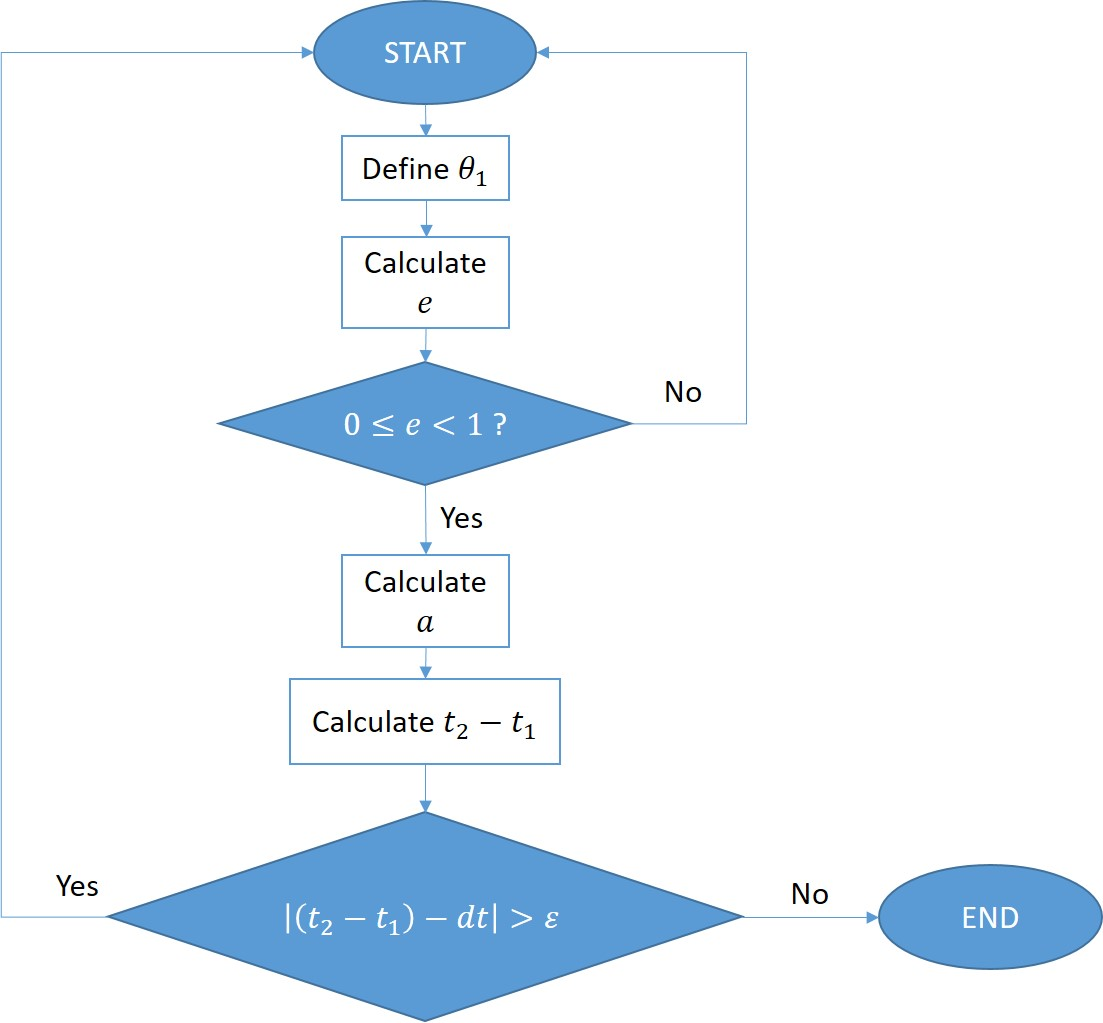
\includegraphics[width=0.8\textwidth]{././images/flowcharteliptic.jpg} 
\caption{Flow chart for the elliptic trajectory resolution.}
\label{Floweliptic}
\end{figure}
\item Hyperbolic trajectory: The equations of the hyperbolic trajectory are:
\begin{equation}
e=\frac{r_2-r_1}{r_1\cos\theta _1-r_2\cos(\theta_1+\Delta\theta)}
\end{equation}
\begin{equation}
a=\frac{r_1\left(1+e\cos\theta _1\right)}{e^2-1}
\end{equation}
\begin{multline}
t_2-t_1=\frac{365.25}{2\pi}a^\frac{3}{2}\Bigg( \frac{e\sqrt{e^2-1}\sin (\theta _1 +\Delta\theta)}{1+e\cos (\theta _1+\Delta\theta)} - \\
ln \left| \frac{\tan \frac{\theta _1 +\Delta\theta}{2}+\sqrt{\frac{e+1}{e-1}}}{\tan \frac{\theta _1 +\Delta\theta}{2} -\sqrt{\frac{e+1}{e-1}}} \right| -\frac{e\sqrt{e^2-1}\sin \theta _1}{1+e\cos \theta _1}+ln\left| \frac{\tan \frac{\theta _1}{2}+\sqrt{\frac{e+1}{e-1}}}{\tan \frac{\theta _1}{2}-\sqrt{\frac{e+1}{e-1}}}\right| \Bigg)
\end{multline}
The resolution is similar to that of the elliptic case, but the acceptable values of the eccentricity change. The flow chart is shown in Figure \ref{Flowhyp}.
\begin{figure}[H]
\centering
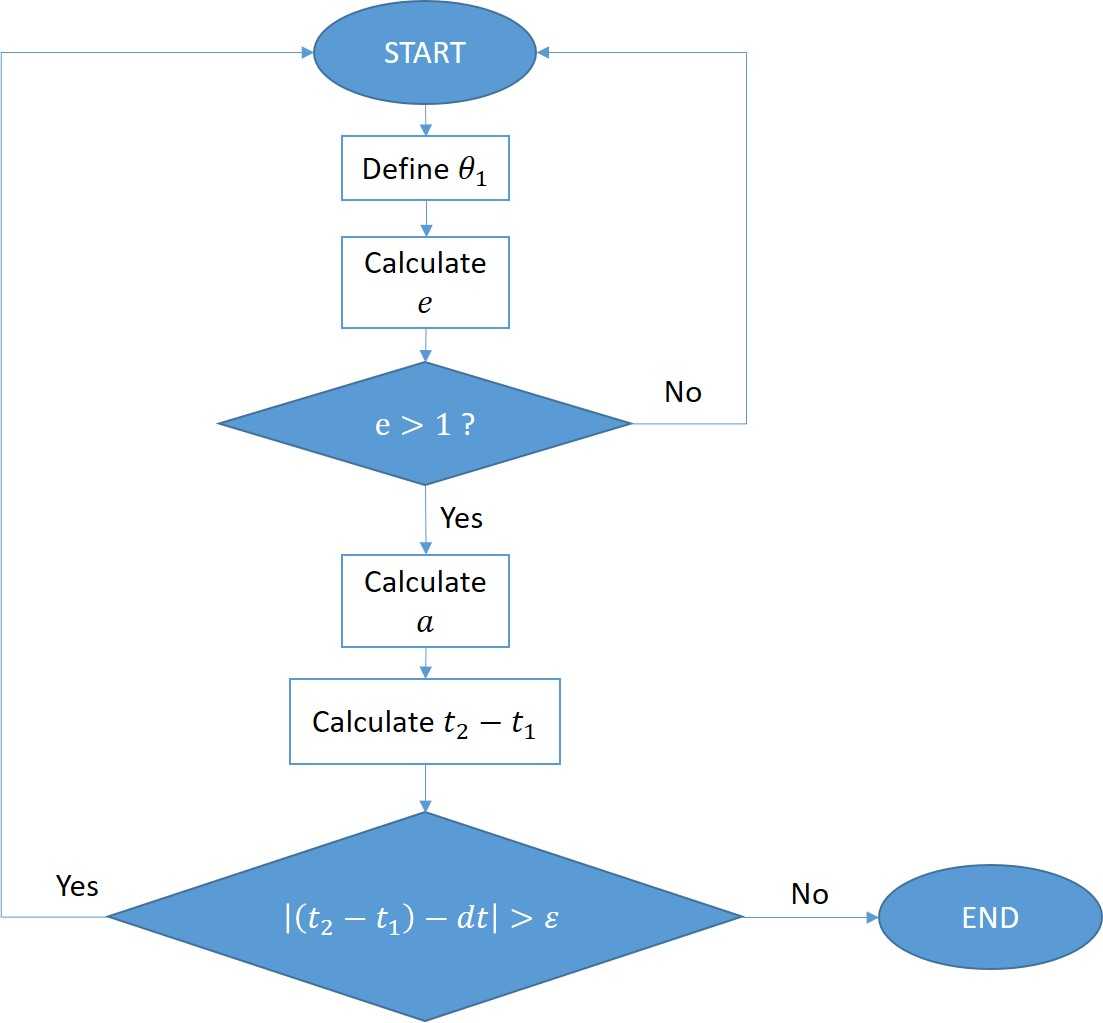
\includegraphics[width=0.8\textwidth]{././images/flowcharthyp.jpg} 
\caption{Flow chart for the hyperbolic trajectory resolution.}
\label{Flowhyp}
\end{figure}
\end{itemize}
\paragraph{Argument of the perihelion} 
The only remaining orbit element that needs to be computed is $\omega$. It can be calculated using results from the previous steps:
\begin{equation}
\omega = 2\pi - (\theta _1 - \sigma )
\end{equation}



\subsubsection{3rd. Planetocentric stage }
\paragraph{} Once the spacecraft, enter into the SOI of the destination planet, the planetocentric stage starts. The spacecraft, describes a planet arrival hyperbola. Depending of the arrival velocity and position three main scenarios can be described for the spacecraft.

\begin{description}
	\item[Impact] If arrival position $r_p \leq R_P$.
	\item[Slowdown] Atmosphere interaction will slowdown the spacecraft if $r_p \leq R_a$.
	\item[Flyby] Spacecraft will perform a flyby over the planet if $r_p > R_a$ or $b > b_a$.	
\end{description}

Note that $R_P$ and $R_a$, correspond to the planet and atmosphere radius respectively.

The spacecraft, will only stay trapped on the destination planet, orbiting, if the spaceship has slowdown enough in contact with the planet atmosphere or the spaceship braked during the periastron.

Because, the main assignment objective was to calculate, a trajectory between to planets for interplanetary travel. This stage is been only develop theoretically, expressions for computing theses parameters can be obtained on, \cite{PCA}. First and third stage of the PCA, share some concepts and equations because in both, an hyperbolic trajectory is performed. 